\documentclass[tikz,border=10pt]{standalone}
\usetikzlibrary{intersections, calc}

\begin{document}
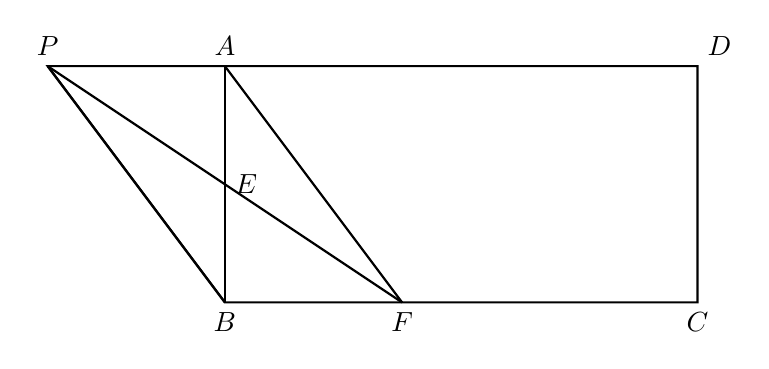
\begin{tikzpicture}[thick, scale=1.5]
    % 1. 定义核心坐标点
    % 设 B 为原点 (0,0)，矩形高度为 2，矩形底边长为 4，P点向左偏移 1.5
    \coordinate (B) at (0,0);
    \coordinate (A) at (0,2);
    \coordinate (C) at (4,0);
    \coordinate (D) at (4,2);
    \coordinate (P) at (-1.5,2);
    \coordinate (F) at (1.5,0); % 点F在BC上

    % 2. 绘制基础图形
    \draw (P) -- (D) -- (C) -- (B) -- cycle; % 矩形 ABCD 及 PBD
    \draw (P) -- (B); 
    \draw (A) -- (F); 
    \draw (P) -- (F);
    \draw (A) -- (B); 

    % 3. 计算交点 E (PF 与 AB 的交点)
    \path [name path=linePF] (P) -- (F);
    \path [name path=lineAB] (A) -- (B);
    \path [name intersections={of=linePF and lineAB, by=E}];

    % 4. 标注点位
    \node[above] at (P) {$P$};
    \node[above] at (A) {$A$};
    \node[above right] at (D) {$D$};
    \node[below] at (B) {$B$};
    \node[below] at (F) {$F$};
    \node[below] at (C) {$C$};
    \node[right] at (E) {$E$}; % 点E位于线段PF和AB的交汇处

\end{tikzpicture}
\end{document}